% ---------------------------------------------------------------------------
% Author guideline and sample document for EG publication using LaTeX2e input
% D.Fellner, v1.13, Jul 31, 2008

\documentclass{egpubl}
\usepackage{eurovis2019}

% --- for  Annual CONFERENCE
% \ConferenceSubmission   % uncomment for Conference submission
% \ConferencePaper        % uncomment for (final) Conference Paper
% \STAR                   % uncomment for STAR contribution
% \Tutorial               % uncomment for Tutorial contribution
% \ShortPresentation      % uncomment for (final) Short Conference Presentation
% \Areas                  % uncomment for Areas contribution
% \MedicalPrize           % uncomment for Medical Prize contribution
% \Education              % uncomment for Education contribution
% \Poster                 % uncomment for Poster contribution
% \DC                     % uncomment for Doctoral Consortium
%
% --- for  CGF Journal
% \JournalSubmission    % uncomment for submission to Computer Graphics Forum
% \JournalPaper         % uncomment for final version of Journal Paper
%
% --- for  CGF Journal: special issue
% \SpecialIssueSubmission    % uncomment for submission to , special issue
% \SpecialIssuePaper         % uncomment for final version of Computer Graphics Forum, special issue
%                          % EuroVis, SGP, Rendering, PG
% --- for  EG Workshop Proceedings
% \WsSubmission      % uncomment for submission to EG Workshop
% \WsPaper           % uncomment for final version of EG Workshop contribution
% \WsSubmissionJoint % for joint events, for example ICAT-EGVE
% \WsPaperJoint      % for joint events, for example ICAT-EGVE
% \Expressive        % for SBIM, CAe, NPAR
% \DigitalHeritagePaper
% \PaperL2P          % for events EG only asks for License to Publish

% --- for EuroVis 
% for full papers use \SpecialIssuePaper
% \STAREurovis   % for EuroVis additional material 
\EuroVisPoster % for EuroVis additional material 
% \EuroVisShort  % for EuroVis additional material

 \electronicVersion % can be used both for the printed and electronic version

% !! *please* don't change anything above
% !! unless you REALLY know what you are doing
% ------------------------------------------------------------------------

% for including postscript figures
% mind: package option 'draft' will replace PS figure by a filename within a frame
\ifpdf \usepackage[pdftex]{graphicx} \pdfcompresslevel=9
\else \usepackage[dvips]{graphicx} \fi

\PrintedOrElectronic

% prepare for electronic version of your document
\usepackage{t1enc,dfadobe}

\usepackage{egweblnk}
\usepackage{cite}

% For backwards compatibility to old LaTeX type font selection.
% Uncomment if your document adheres to LaTeX2e recommendations.
% \let\rm=\rmfamily    \let\sf=\sffamily    \let\tt=\ttfamily
% \let\it=\itshape     \let\sl=\slshape     \let\sc=\scshape
% \let\bf=\bfseries

% end of prologue
% ---------------------------------------------------------------------
% EG author guidelines plus sample file for EG publication using LaTeX2e input
% D.Fellner, v2.02, Jan 25, 2017


\title[Improving the Scalability of Interactive Visualization Systems for Exploring Threaded Conversations]%
      {Improving the Scalability of Interactive Visualization Systems for Exploring Threaded Conversations}

% for anonymous conference submission please enter your SUBMISSION ID
% instead of the author's name (and leave the affiliation blank) !!
% for final version: please provide your *own* ORCID in the brackets following \orcid; see https://orcid.org/ for more details.
\author[A. McNutt \& G. Kindlmann]
{\parbox{\textwidth}{\centering A. McNutt, IEEE student member, \& G. Kindlmann
%        S. Spencer$^2$\thanks{Chairman Siggraph Publications Board}  
        }
        \\
% For Computer Graphics Forum: Please use the abbreviation of your first name.
{\parbox{\textwidth}{\centering Department of Computer Science, University of Chicago
%        $^2$ Another Department to illustrate the use in papers from authors
%             with different affiliations
       } 
}
}
% ------------------------------------------------------------------------

% if the Editors-in-Chief have given you the data, you may uncomment
% the following five lines and insert it here
%
% \volume{36}   % the volume in which the issue will be published;
% \issue{1}     % the issue number of the publication
% \pStartPage{1}      % set starting page


%-------------------------------------------------------------------------
\begin{document}

\teaser{
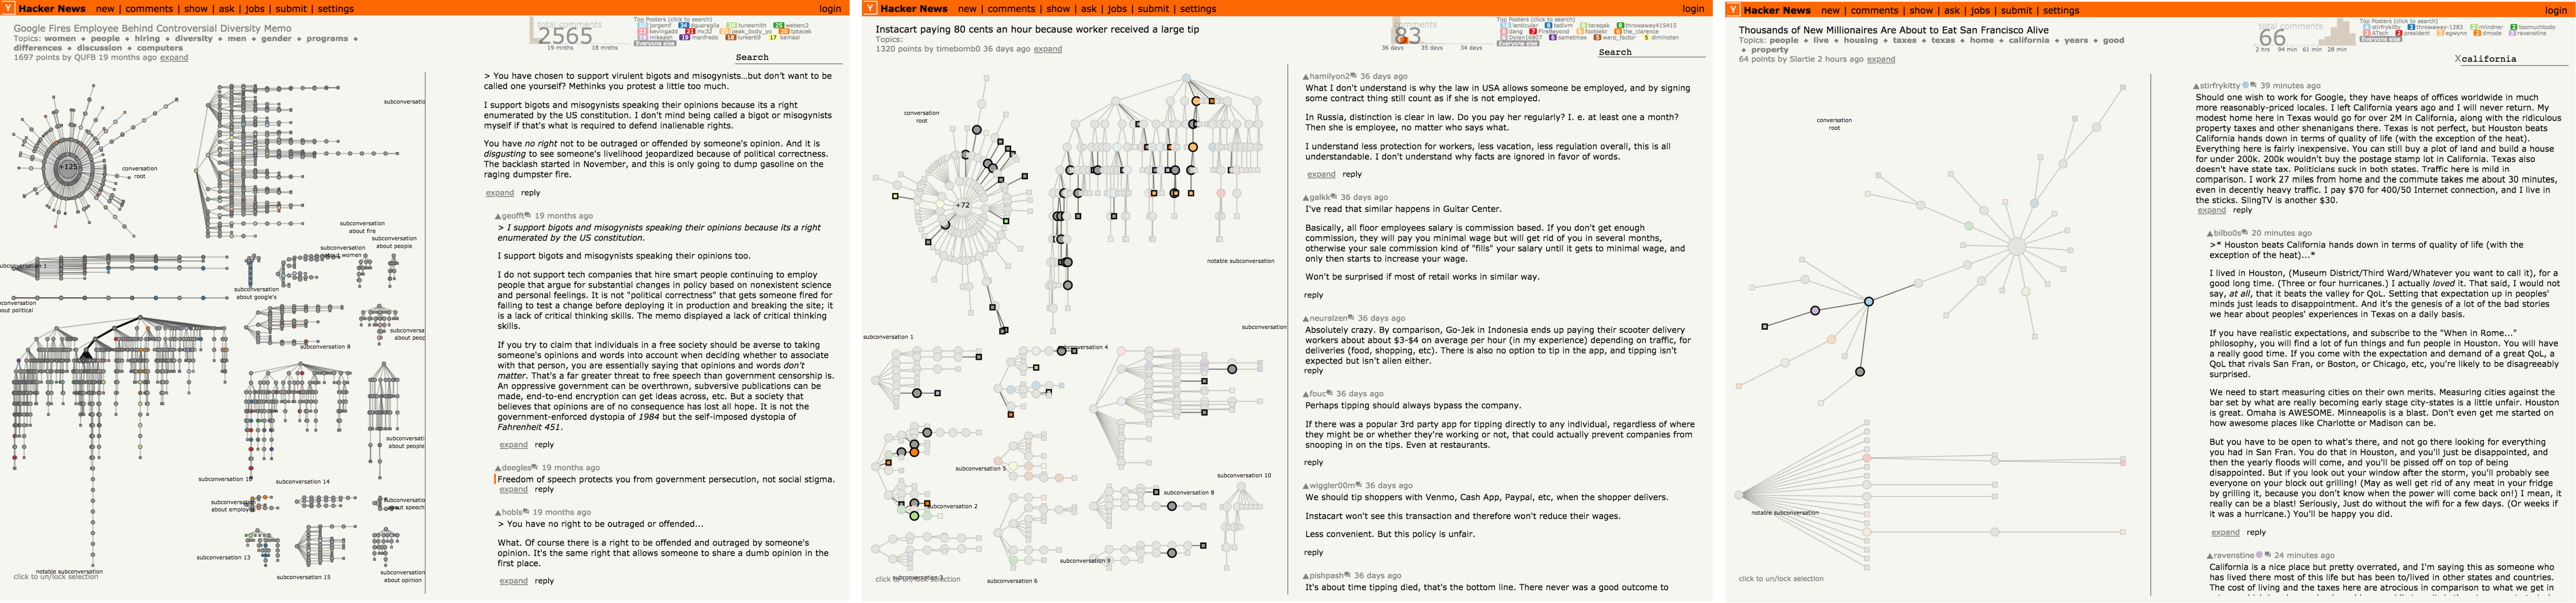
\includegraphics[width=\linewidth]{images/teaser.pdf}
\centering
\caption{
Two HackerNews conversations (715 and 85 comments respectively) rendered using our ForumExplorer application.
%
In the left image the user has moused over a particular sub-conversation; in the right they have engaged in a temporal search.
}
\label{fig:teaser}
}

\maketitle
%-------------------------------------------------------------------------
\begin{abstract}
There has been a variety of works on developing visualization systems to augment and enhance the experience of interacting with the threaded conversations found in venues like reddit and slashdot through the use of graphical overview and nlp-generated summaries.
%
These works have generally been designed around an ideal size of data, which can be difficult to use for large conversations, and have sometimes require non-trivial offline processing time.
%
In tandem these factors have likely negatively affected the adoption of this class of tool.
%
We address these problems by offering concrete design strategies that enable this type of representation to handle wider ranges of data, that we implement as a Chrome Extension, Forum Explorer, which facilitates practical real-time analysis and exploration of conversations held on yCombinator's HackerNews.
%   The ABSTRACT is to be in fully-justified italicized text, 
%   between two horizontal lines,
 %  in one-column format, 
%   below the author and affiliation information. 
 %  Use the word ``Abstract'' as the title, in 9-point Times, boldface type, 
  % left-aligned to the text, initially capitalized. 
 %  The abstract is to be in 9-point, single-spaced type.
  % The abstract may be up to 3 inches (7.62 cm) long. 
  \\
%   Leave one blank line after the abstract, 
%   then add the subject categories according to the ACM Classification Index 
%-------------------------------------------------------------------------
%  ACM CCS 1998
%  (see http://www.acm.org/about/class/1998)
% \begin{classification} % according to http:http://www.acm.org/about/class/1998
% \CCScat{Computer Graphics}{I.3.3}{Picture/Image Generation}{Line and curve generation}
% \end{classification}
%-------------------------------------------------------------------------
%  ACM CCS 2012
%   (see http://www.acm.org/about/class/class/2012)
%The tool at \url{http://dl.acm.org/ccs.cfm} can be used to generate
% CCS codes.
%Example:
\begin{CCSXML}
<ccs2012>
<concept>
<concept_id>10010147.10010371.10010352.10010381</concept_id>
<concept_desc>Human-centered computing~User interface design</concept_desc>
<concept_significance>300</concept_significance>
</concept>
<concept>
<concept_id>10010583.10010588.10010559</concept_id>
<concept_desc>Human-centered computing~Visualization</concept_desc>
<concept_significance>200</concept_significance>
</concept>
<concept>
<concept_id>10010583.10010584.10010587</concept_id>
<concept_desc>Human-centered computing~Graph drawings</concept_desc>
<concept_significance>100</concept_significance>
</concept>
</ccs2012>
\end{CCSXML}

\ccsdesc[300]{Human-centered computing~User interface design}
\ccsdesc[200]{Human-centered computing~Visualization}
\ccsdesc[100]{Human-centered computing~Graph drawings}


\printccsdesc   
\end{abstract}





%-------------------------------------------------------------------------
\section{Introduction}


%%%
%%% Figure 1
%%%
\begin{figure}[htb]
\centering
% the following command controls the width of the embedded PS file
% (relative to the width of the current column)
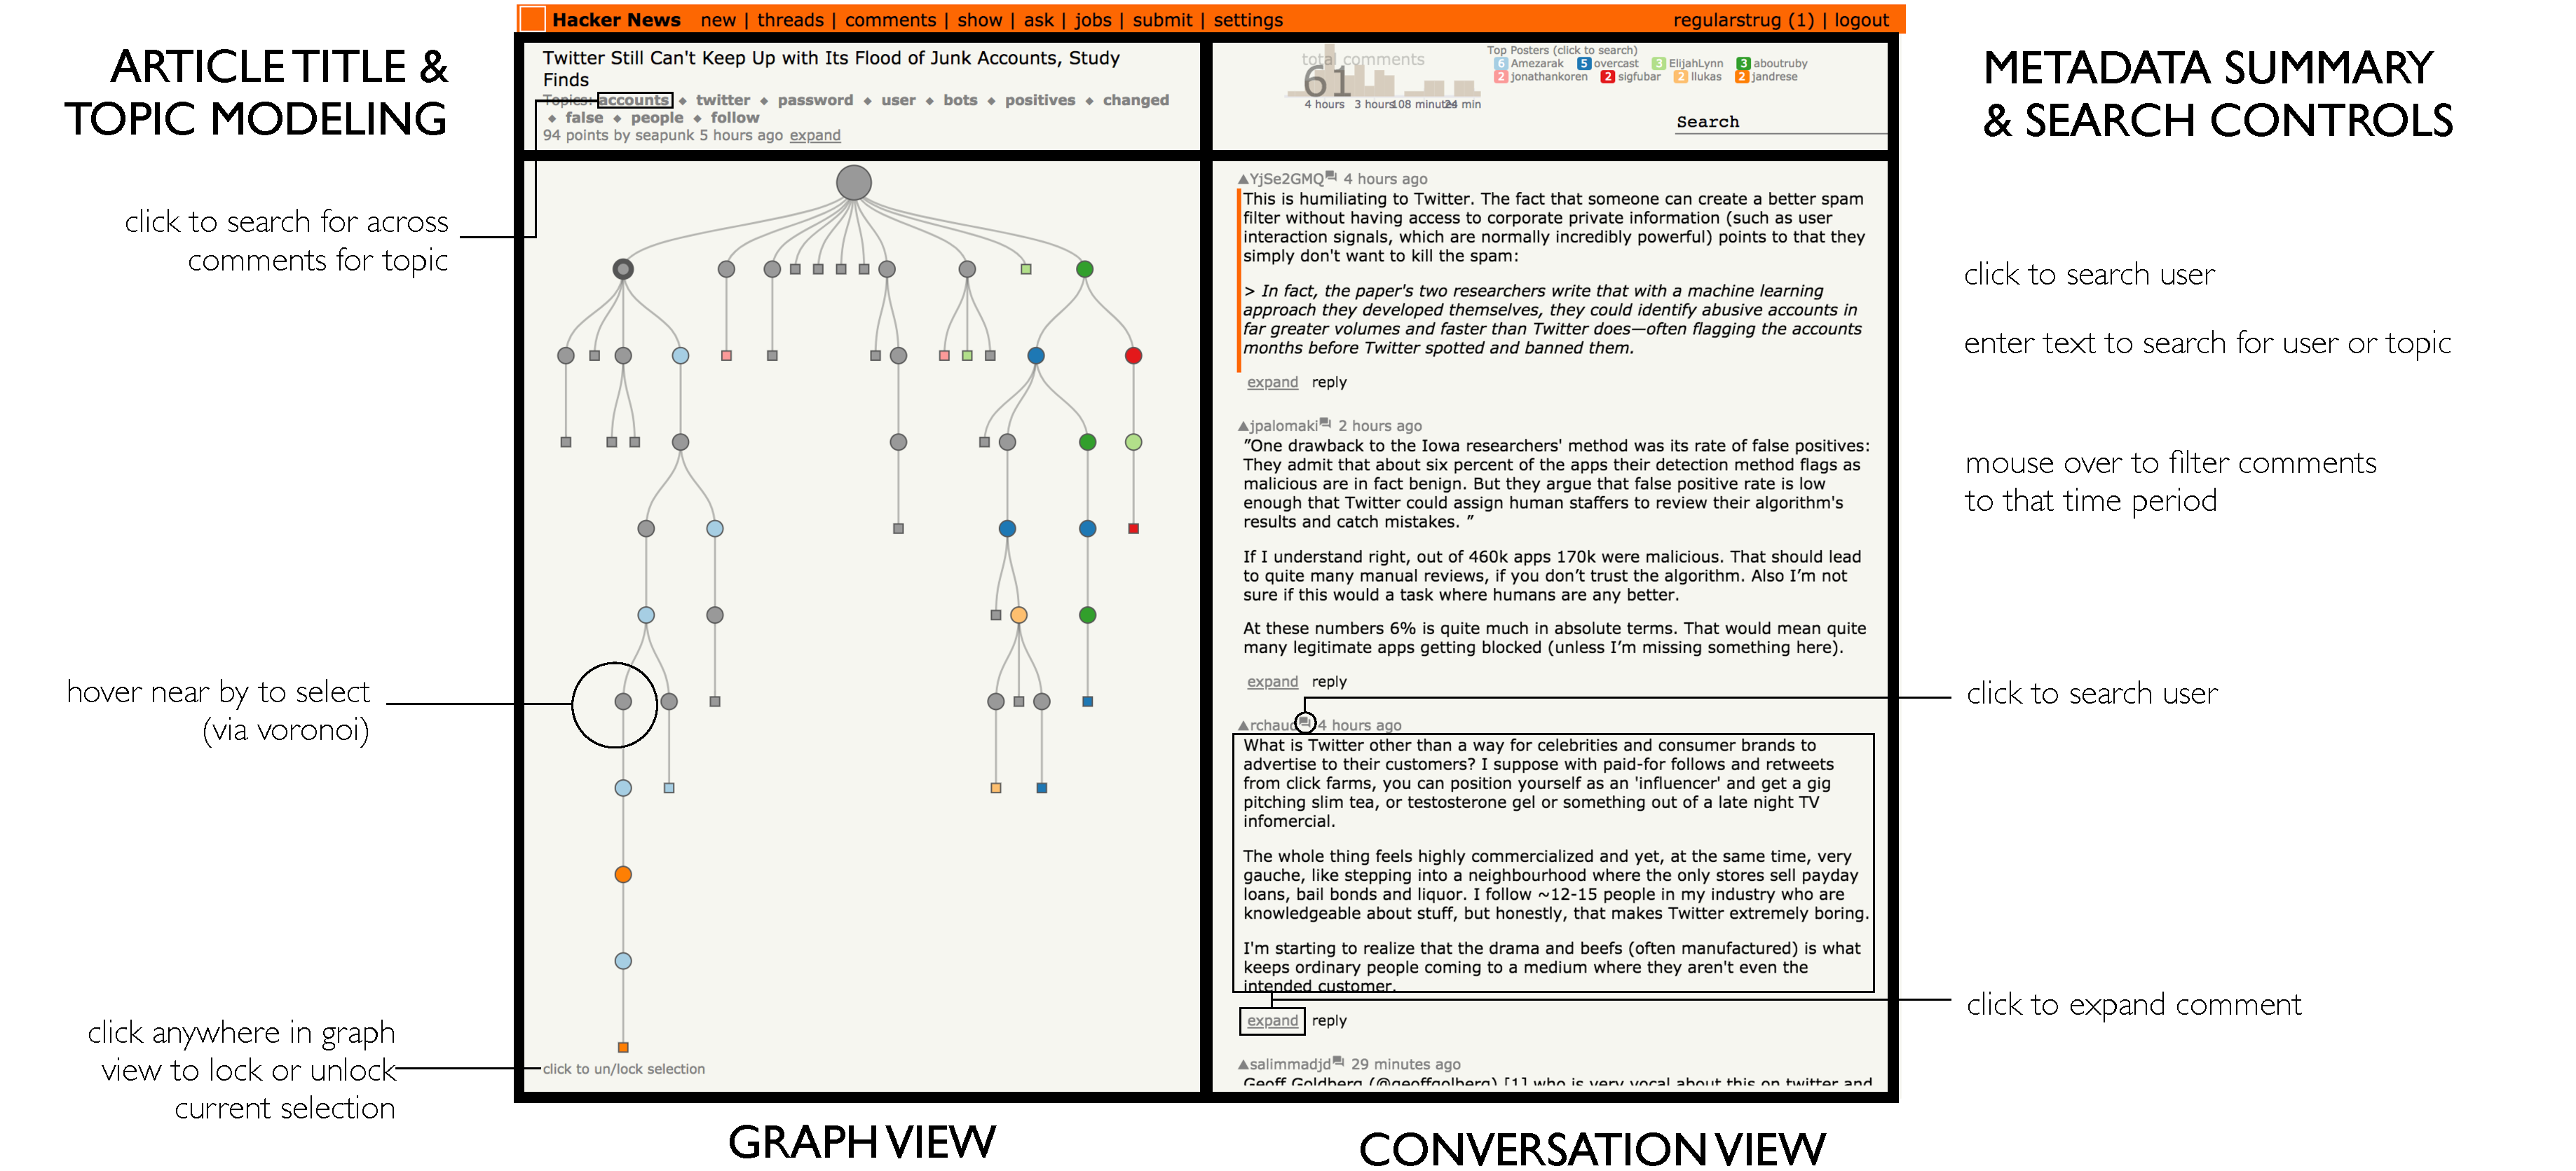
\includegraphics[width=\linewidth]{images/explainer.pdf}
% replacing the above command with the one below will explicitly set
% the bounding box of the PS figure to the rectangle (xl,yl),(xh,yh).
% It will also prevent LaTeX from reading the PS file to determine
% the bounding box (i.e., it will speed up the compilation process)
% \includegraphics[width=.95\linewidth, bb=39 696 126 756]{sampleFig}
%
%  \parbox[t]{.9\columnwidth}{\relax
%          For all figures please keep in mind that you \textbf{must not}
%         use images with transparent background! 
%         }
%
\caption{
\label{fig:explainer}
Annotated view explaining the components of the UI. In addition to our Forested Tree View we support Reingold-Tilford tidy tree (both as a ring and linear tree) and gridded tree views.
}
\end{figure}


Conversation on the internet takes many shapes and forms, including question and answer forums, synchronous messaging, and asynchronous threaded conversation. 
%
Of particular interest are conversations that take place in an asynchronous threaded environments, such as reddit or slash dot, in which users are presented the opportunity to comment on the root of the conversation or on any previous comments. 
%
These forums offer a mechanism for communities to have wide collections of related conversations within a single topic.
%
In many cases the participants in these conversations are experts on the topic and might provide valuable insights.
%
Unfortunately the design of these digital spaces typically do not allow for users to interact with the conversational corpus as a whole, which can limit or impede understanding of the community opinions and insights about a topic.



%Building systems that provide an overview of a complex or non-linear data space is a favorite class of problems in the information visualization community, and threaded conversations have been no exception.
%
Previous visualization works have developed a fascinating collection of UI paradigms to address this space. 
%
A common trend among these works features a overview of the conversational thread encoded as a graph-like structure, which the user then interacts with in a details-on-demand \cite{shneiderman1996eyes} pattern to expose components of the discourse. 
%
While these tools are uniformly well received by their evaluation audiences, they have failed to gain widespread usage.
%
This may be because visualization based overview systems are not well aligned with the types of tasks that people pursue on threaded forums.
%
Optimistically we hope that visualization might provide helpful solutions, and that previous iterations have failed to gain traction because they do not possess an accessible or online implementations, are not aligned to the specific community they are trying to affect, and are designed around a single ideal size of conversation (and thus become cumbersome or difficult to use when conversations of interest fall outside of that target domain). 







\section{Forum Explorer}

We present Forum Explorer, a Chrome Extension that repurposes the conventional layout of yCombinator's HackerNews \cite{hackernews} to facilitate better data exploration through the use of tree visualization techniques.
%
We implement a split pane view in which simultaneously shows a graphical overview and a detail view. 
%
We provide additional detail about the UI in Figure \ref{fig:explainer}. 
%
We support sub-conversational discovery by coloring vertices corresponding to the dozen top commenters, which allows for easy identification and exploration of conversations between individuals in the midst of this dialog.
%
% The application is implemented using d3, redux, react, and react-vis.
%
We provide topic model summaries of the conversation through the use of Latent Dirichlet Allocation (via lda.js \cite{lda-js}), which we compute on a caching micro-service hosted on Heroku. 
%



Our system expands upon previous work through a pair of novel visual encodings.
%
Firstly, we introduce a novel Forested Tree View which splits threaded conversations at the root into a collection of smaller and more legible trees, by observing that the weights of rooted branches tends to be heavily dominate by a small collection of sub-trees.
%
We prune the heaviest branches from the root and present them as independent trees, which organize in space by computing a SliceDice treemap consisting for a fake tree consisting of the weights of the rooted and the pruned trees.
%
This approach allows for ample visual space to provide in-situ annotations and textual guides. 
%
We find empty space in the visualization to add these annotations (which we supply as topic model summaries) by constructing a voronoi for the total layout, and then finding the largest (and hence emptiest) cell for each subtree of the layout.
%
Secondly, we observe that large conversations tend to be have a large number of rooted stumps that add substantial visual noise.
%
We address this by collapsing rooted stumps into the root, while still making those nodes accessible through a details on demand interaction.



% TODO NEED TO SCRAPE HACKERNEWS TO FIGURE OUT MAX COMMENT THREAD


%The graphical overview consists of a one of a collection of tree visualizations (in addition to our Forested View, these include an unsegmented radial layout, a reinfold-something tidy tree CITATION, a gridded tree CITATION, and an orbit layout CITATION)  with the origin comment represents as the root of the tree. 
%






 
 \section{Related Work}
 
 Previous work on this topic has developed a number of different strategies for displaying and facilitating novel user interactions under a variety of different design goals.
 %
 The first work of this type appears to be Donath et al's Loom, which introduced the idea of graphical exploration of comment graphs \cite{donath1999visualizing}. 
 %
 This was followed by Sack's Conversation Map which represented conversation as a tree-like structure \cite{sack2000conversation}. 
 %
 Watternberg et al present a pair of papers which introduced split pane view, with one providing the graphical overview (which mirrored the multiply-indented form that threaded conversation are usually depicted in) and the other displaying comments \cite{wattenberg2003conversation, dave2004flash}.
% 
Pascual-Cid et al introduce a space filling radial tree layout \cite{pascual2009exploring}. 
%
Narayan construct tldr which focuses on reddit and encodes the tree as an icicle diagram \cite{narayan2010not}. 
%
Hoque et al's family of tools breaks from purely metadata visualization by adding topic modeling and sentiment analysis on top of a split pane interaction with an abstracted indentation view \cite{hoque2014convis, hoque2016interactive}.
%
Each of these tools provide valuable insight, but come at the cost of forcing their users to use an unfamiliar environment, as well as being not being actually deployed.
%
Most closely related to our technical approach is Treeverse, a chrome extension which allows users to visualize the conversation tree associated with a particular tweet \cite{treeverse}.
%
 Our work improves over this design in that it tightens the response interaction response cycle and enables the user to extract useful information from a single view, as well as being better matched with the domain target audience.


%-------------------------------------------------------------------------
\section{Conclusions \& Future Work}

We have presented Forum Explorer, a tool for exploring threaded conversations on HackerNews. 
%
Our primary contribution is a novel Forested Tree layout that facilitates better scalability for systems of this type, however we believe that there is substantial room for our tool to make contributions in the future.
%
Previous studies of threaded conversations usefully demonstrate the general usability of the constituent structural design elements.
%
Yet it is unclear from their results whether or not these results are due to the novelty of the systems, and therein experiment bias (as noted by Isenberg et al is a frequent result of the visualization communities user studies \cite{isenberg2013systematic}), or the true usefulness of the tool.
%
The best evidence that this type of system has substantive utility (beyond Treeverse's modest popularity, as evidenced by 2412 active installs at the time of this writing) is that it used by Rao et al \cite{twittercanoes} to study the way that twitter is used within siloed domain specific knowledge sharing discussions.
%
Our application is well positioned, as it operates in real time, to conduct a longitudinal study that could describe might interact with this type of tool when they are able to incorporate it into their day to day workflow.
%
The strategies described here continue the on-going dialog in the vis community on this topic, but we believe that they could also have applicability to systems outside of threaded conversations, such as visualizations of the scholarly citation graph.



% While these studies usefully demonstrate the usability of the structural design elements in general, their context as laboratory based analyses precludes them from providing longitudinal information about the way users might interact with this type of tool when they are able to incorporate it into their day to day workflow. Forum Explorer is well positioned 

% Our current design process has, in the lens of data feminism, been unfeminist. Our design process happened without consultation of those who might find the application (other than perhaps ourselves). While we are able to rest on the many of the observations from ConVis's prior user studies in the topic, individual forum users tend to have individual expectations about their tools.

% The specific utility of this type of conversation overview tool remains unclear, the lessons learned from ours and other systems could readily be applied to graph analysis problems of a similar size and scale. Analysis of locally relevant articles in the scholarship graph are one such example of this type of system.




%-------------------------------------------------------------------------

%\bibliographystyle{eg-alpha}
\bibliographystyle{eg-alpha-doi}

\bibliography{forum-bib}

\end{document}

